The objective for training deep learning models is to reduce
the error in prediction on each iteration and 
learn data patterns and relationships by increasing the 
prediction accuracy. Cost function is an appropriate method to 
analyse the performance of the neural network as it describes 
how well, model is predicting the actual results. The equation below 
describes the cost function equation also known as mean squared error \citep{7013173}.
\vspace{2mm}

\begin{center}
\begin{equation}
    c = \frac{1}{2m} \sum_{i=1}^m(h - y)^2
\end{equation}
\end{center}

In, equation(1.2)  h is the predected outcome of the intelligent model 
and y is the actual value of the input. The equation above is mean square of 
predected value - actual value. The objective of optimisation algorithms is 
minimise the equation(1.2) to decrease the value of cost function so, the value is 
close to zero as much as possible so, that predected and actual 
value are almost same which means overall model accuracy has improved \citep{7013173}.

\begin{figure}[!htp]
    \centering
    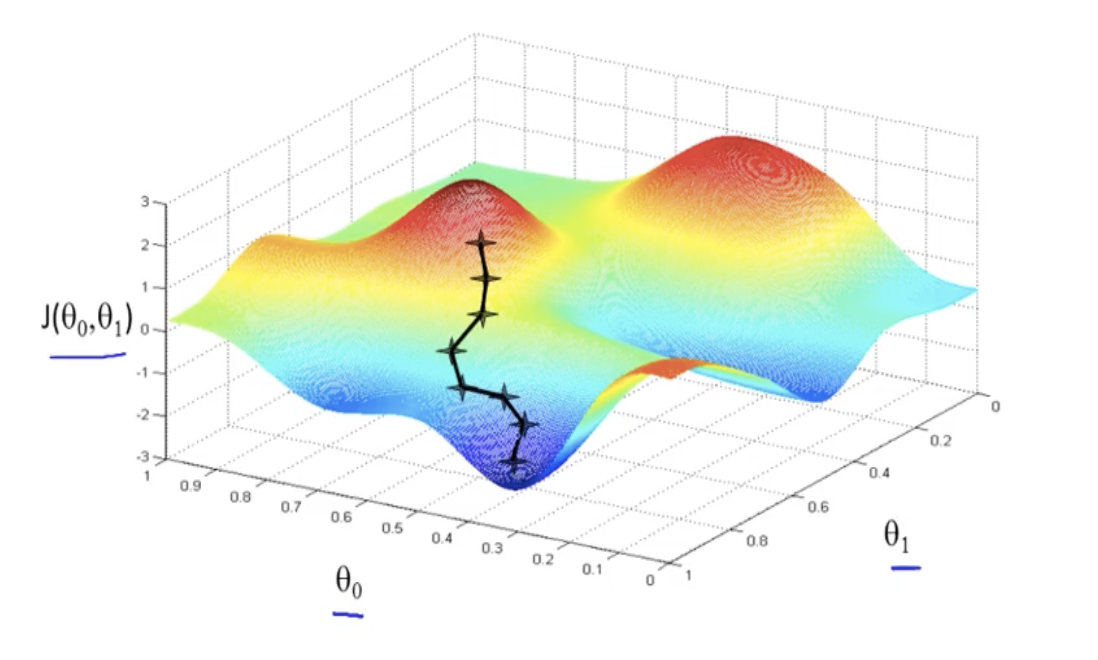
\includegraphics[width=\textwidth]{Images/gd.png}
    \caption{Gradient Descent}
\end{figure}

Gradient descent algorithm  is a optimisation algorithm which is iterative in nature aims 
to minimise the cost function is gradient descent. The algorithm functions by minimising the objective 
function in the space. 

\begin{center}
    \begin{equation}
            \frac{\partial }{\partial w} (\frac{1}{2m} \sum_{i=1}^m(h - y)^2)
    \end{equation}

    \begin{equation}
        \frac{\partial }{\partial b} (\frac{1}{2m} \sum_{i=1}^m(h - y)^2) 
    \end{equation}
\end{center}


The algorithm functions by finding the 
partial deravative of the cost function in respect to weights and bias as shown in the equations (1.3) and  (1.4) above.
The objective is to find minmum of the cost fuction which improves the accuracy \citep{7013173}. 
Backpropagation utilises the gradient descent algorithm and propgates after each layer to 
update the bias and weights in backwards direction to improve accuracy of the model.
